\subsubsection{Components}
To manage the components, EmporioLambda uses React, a Javascript\textsubscript{G} and Typescript\textsubscript{G} library. This allows us to create user-interfaces and UI components.
There are 2 main types of components:
\begin{itemize}
\item \textbf{Presentational Components:} they don't use any state or function. Their only purpose is to show data or call functions from higher level components. Every presentational component can only have children of the same type;
\item \textbf{Container Components:} they can use state variables and functions for their management. They also don't have any restriction about the type of their children.
\end{itemize}
The use of these 2 different components introduces us to the first design pattern used by EmporioLambda: the \textbf{presentational and container components pattern}. This pattern allows us to create a page by using only single components, each with their own responsibility. This also easily lets us separate the \textit{presentational logic} and the \textit{business logic} of the software.\\
React container components can accept 2 variables on their creation:
\begin{itemize}
\item \textbf{props:} variables or objects that can be passed upon component creation by other components;
\item \textbf{state:} variables whose change cause the component to re-render. Its value must be initialized from the component constructor and is read-only.
\end{itemize}
Presentational components can only accept the props variable.\\
The use of the state variables introduces the second design pattern used by EmporioLambda: the \textbf{observer pattern}. This pattern isn't manually implemented by us, as it is a native React pattern. In our case the state of the component is our \textit{observable}: the component, when the state has been changed, automatically re-renders the page with the new values, re-rendering its children as well.\\More information about the observer pattern can be found on this page:\\
\url{https://en.wikipedia.org/wiki/Observer_pattern}.\\

The following diagrams will show the structure of every page, adapted to the UML syntax. The presentational and container components will be recognized by their colors: blue for the first, red for the latter. 

\begin{figure}[H]
\centering
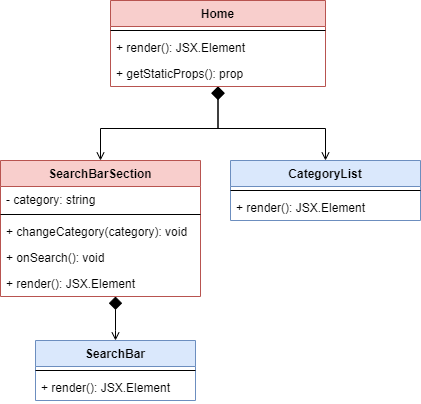
\includegraphics[scale=0.50]{res/Architettura/Frontend/img/home}\\
\caption{Front-end\textsubscript{G} homepage component diagram}
\end{figure}

\begin{figure}[H]
\centering
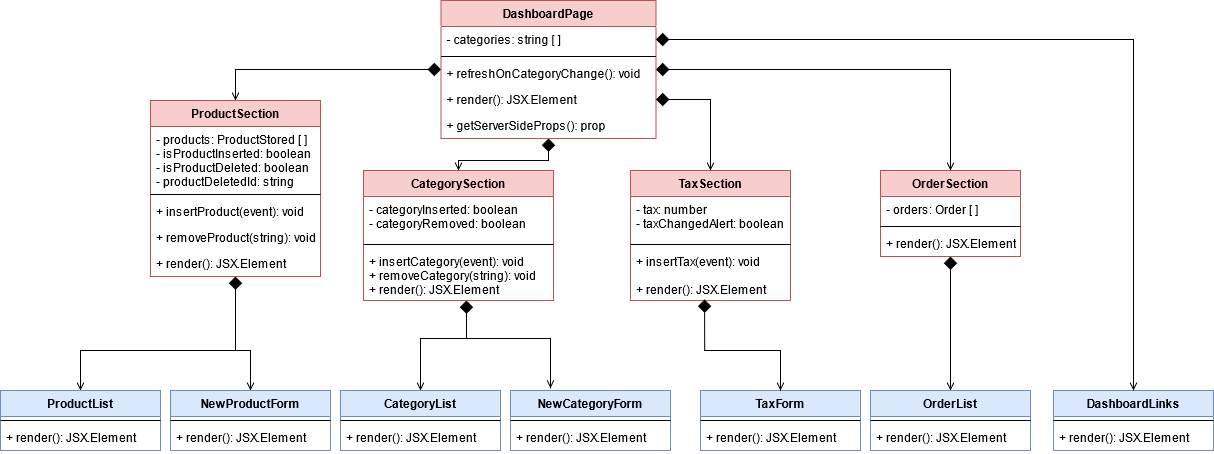
\includegraphics[scale=0.40]{res/Architettura/Frontend/img/dashboard}\\
\caption{Front-end\textsubscript{G} dashboard page component diagram}
\end{figure}

\begin{figure}[H]
\centering
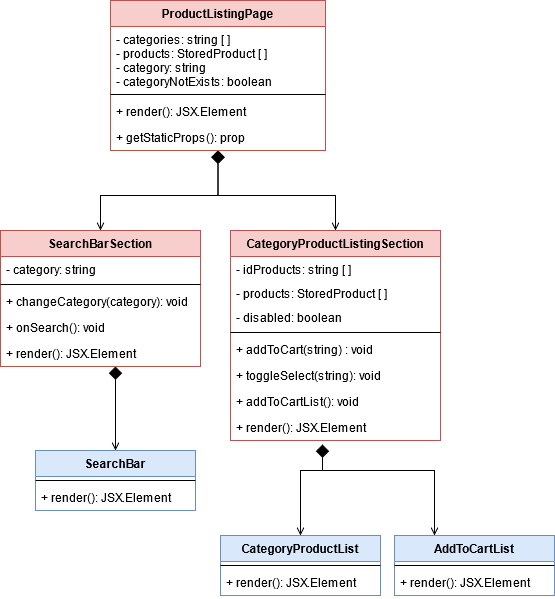
\includegraphics[scale=0.50]{res/Architettura/Frontend/img/plp}\\
\caption{Front-end\textsubscript{G} products listing page component diagram}
\end{figure}

\begin{figure}[H]
\centering
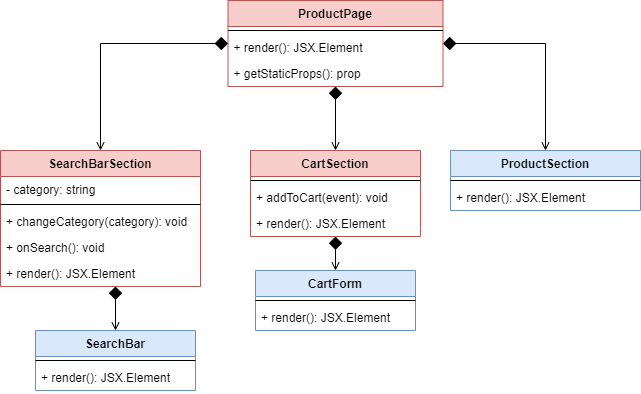
\includegraphics[scale=0.50]{res/Architettura/Frontend/img/pdp}\\
\caption{Front-end\textsubscript{G} product details page component diagram}
\end{figure}

\begin{figure}[H]
\centering
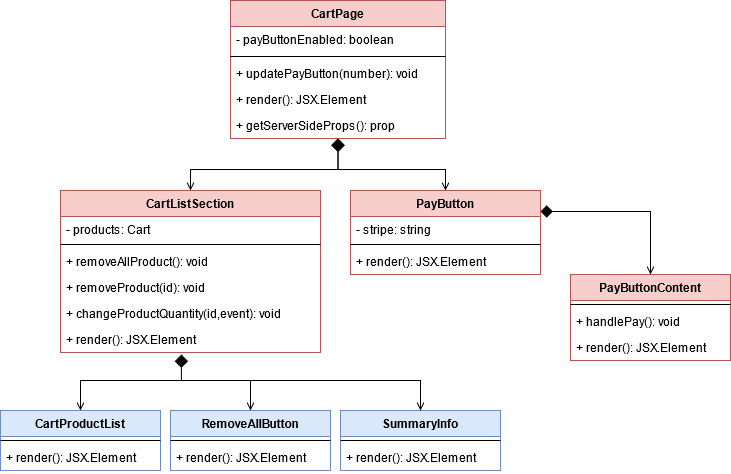
\includegraphics[scale=0.50]{res/Architettura/Frontend/img/cart}\\
\caption{Front-end\textsubscript{G} cart page component diagram}
\end{figure}

\begin{figure}[H]
\centering
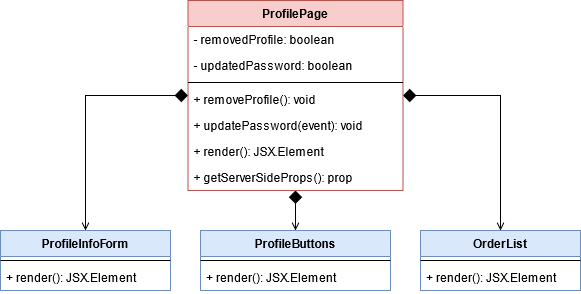
\includegraphics[scale=0.50]{res/Architettura/Frontend/img/profile}\\
\caption{Front-end\textsubscript{G} profile page component diagram}
\end{figure}

\begin{figure}[H]
\centering
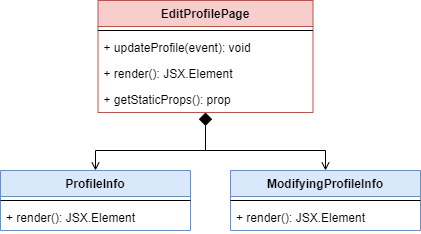
\includegraphics[scale=0.50]{res/Architettura/Frontend/img/editProfile}\\
\caption{Front-end\textsubscript{G} edit profile page component diagram}
\end{figure}

\begin{figure}[H]
\centering
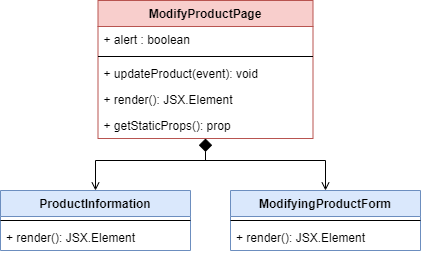
\includegraphics[scale=0.50]{res/Architettura/Frontend/img/modifyProduct}\\
\caption{Front-end\textsubscript{G} edit product page component diagram}
\end{figure}

\begin{figure}[H]
\centering
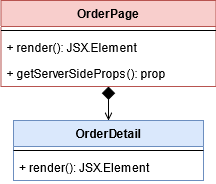
\includegraphics[scale=0.50]{res/Architettura/Frontend/img/order}\\
\caption{Front-end\textsubscript{G} order details page component diagram}
\end{figure}

\begin{figure}[H]
\centering
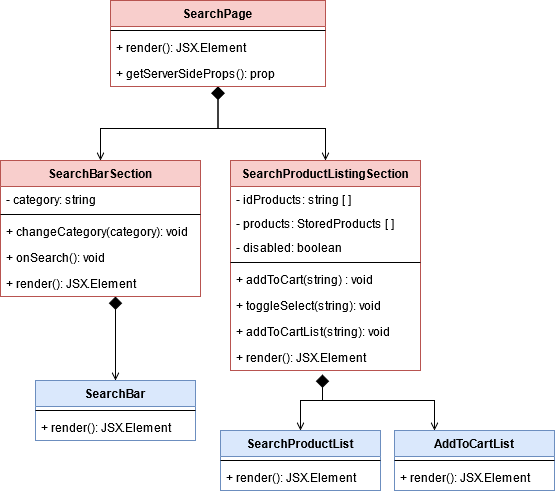
\includegraphics[scale=0.50]{res/Architettura/Frontend/img/search}\\
\caption{Front-end\textsubscript{G} search page component diagram}
\end{figure}

